\chapter{Marco teórico referencial de la investigación}\label{chap:1}

En el presente capítulo se muestran algunos de los principales problemas asociados a la formación de equipos, en particular se estudian los casos de equipos para el desarrollo de proyectos de software, la alineación de un equipo de béisbol y la formación de los colectivos de asignaturas para la distribución de la carga docente en un período lectivo determinado. Además, se abordan los conceptos referentes a esta problemática y, se realiza una explicación detallada del problema a resolver.

\section{Marco teórico referencial de la investigación}

Desde tiempos remotos los seres humanos han trabajado en equipo para afrontar diversas situaciones. Para esto, se dividían el trabajo entre todos sus integrantes, asignándole a cada uno lo que mejor sabía hacer. Hoy en día la asignación de personas a un equipo para solucionar o enfrentar un problema, resulta de gran importancia y de alta complejidad. Esto se debe a la gran cantidad de combinaciones posibles entre todos los factores a tener en cuenta. Existen diferentes conceptos a tener en cuenta para entender este problema. Así, es preciso exponer algunos conceptos claves para el desarrollo de este trabajo.

\subsection{Conceptos fundamentales}

%Un proyecto, según la definición expuesta en \cite{Institute2020}, “es un esfuerzo temporal que se lleva a cabo para crear un producto, servicio o resultado único”. Es decir, un proyecto tiene un tiempo de vida definido, y como resultado de él, se obtiene un producto específico.\\

En \cite{63} se plantea que un equipo consiste en, al menos dos personas trabajando por un objetivo común, donde cada una tiene asignado roles, y que, para completar su objetivo existe dependencia entre sus integrantes.\\

Según \cite{64} un rol “es un puesto que puede ser asignado a una persona o conjunto de personas que trabajan juntas en un equipo, y que requiere habilidades y responsabilidades como: realizar determinadas actividades y desarrollar determinados artefactos”. Los miembros de un equipo pueden ocupar varios roles y un mismo rol puede ser ocupado por varios miembros del equipo \citep{Mayi09}.\\

Las competencias son características de las personas, que se evidencian cuando desempeñan alguna tarea, tienen que ver con la ejecución exitosa de esta, tienen una relación causal con el rendimiento laboral y pueden ser generalizables a más de una actividad \cite{Boyatzis1982}. En este trabajo se distinguen dos tipos o familias de competencias \citep{Mayi09, 76}:
\begin{itemize}
	\item  “Genéricas, también llamadas transversales, claves o capacidades de comportamiento, las cuales definen las características referidas al comportamiento general del empleado, independientes de los conocimientos técnicos específicos. Algunos ejemplos son la capacidad de negociación, el liderazgo y la capacidad de análisis".
	\item  “Técnicas o específicas, las cuales están asociadas a conocimientos y habilidades técnicas específicas de cada puesto de trabajo".
\end{itemize}

Existen diversos tipos psicológicos, los cuales son utilizados para describir o catalogar el carácter de las personas. Para determinar a qué tipo psicológico pertenece una persona se realizan diferentes test, entre ellos Myers-Briggs (test que permite identificar el tipo psicológico de una persona entre los 16 tipos posibles \citep{117, 119}, test de Belbin (test que permite identificar la preferencia por los denominados nueve roles de equipo, divididos en tres categorías: mentales (cerebro, monitor evaluador, especialista), acción (impulsor, implementador y finalizador), sociales (investigador de recursos, cohesionador, coordinador)) y 16 Factores de la Personalidad (test donde se miden 16 factores de personalidad \citep{118}).

\subsection{Formación de equipos de proyectos de software}

En 2020, el informe anual del \textit{Standish Group}\footnote{Firma internacional independiente de asesoría en investigación de las tecnologías}\cite{Group2020} reportó que solamente el 31\% de los proyectos de software culminan con éxito. En este informe se plantea que una de las principales causas del fracaso es la incompetencia de algunos miembros del equipo. Finalmente se llega a la conclusión que la selección de miembros competentes como parte del equipo puede reducir el riesgo de fracaso del proyecto.\\

El problema detectado por \textit{Standish Group}, no es algo nuevo ni reciente. Acompaña a la industria del desarrollo de software desde sus inicios \cite{ElEmam2008}. Es por este motivo que muchos investigadores han dedicado gran parte de su trabajo en búsqueda de perfeccionar este proceso. Por ejemplo, en \cite{Mayi09}, los autores definen un modelo donde queda plasmada la información necesaria a gestionar para el problema. Este modelo toma en cuenta factores que contribuyen a la asignación individual a los roles del proyecto y a la formación del equipo como un todo. Además se propone una herramienta denominada: TEAMSOFT$^+$, que brinda soporte a este modelo.\\

Sin embargo, tanto el modelo presentado en \cite{Mayi09} como la herramienta que le brinda soporte, fueron diseñados para formar un solo equipo; esto limita su uso cuando se desean formar múltiples equipos de proyecto. Utilizar la herramienta desarrollada para dar solución a las situaciones anteriores implicaría formar los equipos de uno en uno (de forma secuencial). Como resultado, los primeros equipos muy buenos y los últimos, serían malos. Dado que en cada iteración se seleccionan los mejores candidatos disponibles, los equipos formados estarían muy  desbalanceados. En el año 2018, tomando en cuenta los trabajos desarrollados sobre el tema, se definió un nuevo modelo que permite la formación de múltiples equipos de proyecto. El modelo toma en cuenta las cuatro funciones objetivos consideradas en \cite{Mayi09} (maximizar competencias, minimizar incompatibilidades, balancear la carga de trabajo y minimizar el costo de desarrollo a distancia) e incorpora funciones como maximizar el interés por desempeñar el rol y maximizar la presencia de roles de Belbin. Además se agregan: maximizar el interés por el proyecto y maximizar la diversidad de tipos MBTI en el equipo \cite{Duran2019}.\\


En \cite{Anagnostopoulos2010} se presenta un marco de trabajo (\textit{framework}) para las tareas de asignación de recursos. Los autores proveen un tratamiento formal sobre cómo representar los equipos y las tareas. Para cada tarea existen un conjunto de habilidades o competencias a tener en cuenta. Mientras que cada persona tiene preferencia sobre las tareas, y ciertas habilidades. El grado de preferencia de las personas por las tareas, y las habilidades que necesitan, pueden configurarse de dos formas, una binaria (si la prefiere o no, expresada con 0 o 1) y una continua (un valor entre 0 y 1).\\


La sabiduría en los equipos de desarrollo de software es un tema poco explotado \cite{Akguen2020}. Sin embargo, \cite{Akguen2020} demuestra que es un factor importante a tener en cuenta en un equipo de desarrollo de software. Esto se debe a que aumenta el desempeño general del equipo y proporciona un mayor conocimiento. El autor define sabiduría como: un proceso donde los miembros del equipo utilizan mejor su conocimiento a través del juicio colectivo, virtudes éticas, emociones/sentimientos y toma de decisiones efectivas durante el proceso de desarrollo del proyecto. Explica también, que existen diversos elementos que influyen en la sabiduría del equipo, por ejemplo: mecanismos (diversidad de los miembros, las relaciones con otros equipos/personas y sus experiencias pasadas) y acciones epistémicas (razonamiento en equipo, intuición). Los resultados de la investigación muestran una asociación positiva entre los elementos de la sabiduría y el proceso y la efectividad del proyecto de desarrollo de software.



\subsection{Formación de equipos en ámbitos docentes}

Otra situación en la que está presente la formación de equipos, es a la hora de asignar profesores a los tipos de clases que le corresponden a las asignaturas. Muchas universidades del mundo tienen que enfrentar este proceso al menos una vez al año. Se han realizado múltiples investigaciones en la literatura enfocándose en la asignación de los profesores a las asignaturas. Por ejemplo, en \cite{Bosquez2020} se propone un modelo para la asignación de asignaturas a profesores, basándose en la preferencia de los mismos hacia las asignaturas (si le interesaba darla o no). En \cite{Domenech2014} se presenta otro modelo, similar al anterior, pero esta vez los autores deciden realizar este proceso asignando los profesores a las asignaturas. Este último tiene en cuenta el balance de la carga de los profesores y sus preferencias hacia las asignaturas.\\

Otro enfoque es el abordado por \cite{AlvaresValedes2002}, donde se desarrolla una solución a este problema, utilizando un algoritmo de búsqueda Tabú. Para esto, en su modelación se tienen en cuenta la disponibilidad de los profesores en cada período de clases. En esta solución los autores descomponen el problema en dos partes. En la primera, asignan los profesores a las asignaturas y grupos de clases. Mientras que en la segunda, se resuelve el problema de horarios resultante. Como resultado muestran que el procedimiento propuesto produce resultados similares o mejores que la asignación proporcionada por otros expertos. A partir de esto, se llega a la conclusión que se puede utilizar conjuntamente con un programa de horarios para resolver todo el problema al que se enfrentan los planificadores en cada curso académico.\\

Existen otros trabajos que se enfocan en la formación de equipos de estudiantes para proyectos escolares. En la literatura se enfatiza la importancia de la composición y el diseño del equipo, y se recomienda que los profesores organicen equipos para asegurar la diversidad de los miembros y un desempeño óptimo. La investigación propuesta por \cite{Pociask2017} los autores se proponen investigar si los diferentes métodos de formación de equipos afectan los resultados del desempeño individual y del equipo, en un curso de pregrado. Para lograr esto los autores diseñan un experimento en tres momentos del curso donde probaron en cada uno tres variantes: equipos construidos por el profesor, por los estudiantes mismos o aleatoriamente por un programa. Como resultado se obtiene que los equipos diseñados por el profesor del curso eran más diversos, pero que los estudiantes de estos equipos no se desempeñaron mejor que los compañeros en equipos autoseleccionados o asignados al azar. Además, debido a que el desempeño de los estudiantes fue similar, independientemente del método de formación de equipos utilizado, los autores sugieren que los equipos formados por los mismos estudiantes pueden ser una opción razonable para que los profesores monten un curso basado en equipos. \\

Otro trabajo relacionado con este tema es el desarrollado por \cite{Kittur2020}, donde los autores analizan y evalúan las prácticas de aprendizaje en equipo. Para ello, utilizan como objeto de investigación a un grupo de curso de pregrado. Los autores se basaron en los resultados obtenidos a partir de la aplicación de un test \cite{Felder}. La aplicación de este cuestionario perseguía el objetivo de obtener las preferencias en los estilos de aprendizaje de los estudiantes, que se dividen en cuatro dimensiones (activo/reflexivo, sensitivo/intuitivo, visual/verbal y secuencial/global). Se formaron los equipos en dos etapas, primero, de forma aleatoria y luego con un balance en las preferencias por los estilos de aprendizaje. Los autores le proporcionaron una problemática a los equipos para conocer el cambio en la comprensión conceptual. A partir de este estudio los autores concluyen que la formación de equipos estratégicos se considera un enfoque favorable para aumentar el aprendizaje de los estudiantes.

\subsection{Formación de equipos de deportes}

La problemática de formación de equipos se extiende también al mundo deportivo. El béisbol, al ser un deporte de equipo, es un ejemplo típico donde se manifiesta esta problemática. Es considerado como uno de los deportes más populares en América y Asia, específicamente en países como: Cuba, Japón, Estados Unidos, entre otros. Sin embargo, en los últimos años, el continente europeo también se ha sumado, teniendo como principales exponentes: Países Bajos, República Checa e Italia \cite{WBSC2021}. Resulta entonces de gran interés la selección de los jugadores para formar un equipo que cumpla con las expectativas de la dirección del equipo y sus fanáticos. Los directores técnicos son los encargados de seleccionar los jugadores que formarán parte de su equipo y de la alineación (defensiva y ofensiva) para cada juego en particular. En este proceso de selección se tiene en cuenta las habilidades y características propias de cada jugador. No son pocos los casos en los que los directores realizan este proceso de forma manual e intuitiva. En \cite{Smith1995} se realiza un estudio sobre las competencias necesarias a tener en cuenta para la formación del equipo. Sin embargo, en la actualidad, las soluciones existentes para este problema \citep{Polyashuk2015, Sugrue2007} no las tienen en cuenta. En estos trabajos, los autores se basan en estadísticas almacenadas de los jugadores a lo largo de los años para construir un indicador. En base a este indicador es que se realiza la asignación. Las investigaciones planteadas anteriormente, solo se enfocan en la formación de la alineación ofensiva (orden al bate), sin tener en cuenta la alineación defensiva.\\

Mientras tanto, \cite{Burney2012} plantea un modelo para elegir la mejor combinación de jugadores de un equipo de criquet. Para realizar la asignación de una persona, los autores crean un indicador (\textit{fitness}). Para calcular este indicador se tienen en cuenta: todos los juegos en los que participa el jugador, y de estos, la cantidad de ganados y perdidos. En \cite{Cooper2009} se propone un nueva forma de medir el desempeño de los jugadores de un equipo de baloncesto, para que los entrenadores lo tengan en cuenta a la hora de decidir qué jugador juega una posición. Mientras que para los equipos de pelota, \cite{Polyashuk2015} y \cite{Sugrue2007} plantean diferentes modelos con un mismo fin, elegir el orden al bate de los jugadores en la alineación inicial, en cada uno se propone una manera distinta de calcular el índice de desempeño de un jugador. Estos modelos se concentran solamente en la solución para la alineación ofensiva, sin tener en cuenta la alineación defensiva. Además, dejan de lado la experiencia, las preferencias de las personas por cada rol y las competencias asociadas a cada uno.


\subsection{Formación de equipos en diferentes áreas}
Los juegos en línea constituyen una fuente importante de interacciones que pueden contribuir a comprender el comportamiento humano. Una posible contribución es comprender qué motiva a las personas a elegir a sus compañeros de equipo. Sobre este tema se centra la investigación planteada en \cite{Alhazmi2017}. Donde los autores utilizan gran cantidad de datos de un entorno de juego en línea basado en equipos, específicamente, \textit{Battlefield 4}\footnote{Popular juego basado en equipos en el que los jugadores eligen uno de los dos equipos competidores para jugar}. Los investigadores definen varios indicadores que influyen en las decisiones de los jugadores para elegir equipo, como son: la familiaridad positiva (si los miembros del equipo han trabajado en ocasiones anteriores con experiencias positivas), la homofilia (tendencia de las personas a buscar otras que son parecidas a ellas) y las competencias. Los autores recolectan la datos de dos meses de interacciones en el juego entre más de 380.000 jugadores. A partir de esto llegan a la conclusión de que la familiaridad es un factor importante en la formación de un equipo, mientras que la homofilia no lo es. Otra conclusión arribada es que las competencias afectan la formación del equipo en mayor forma: los jugadores con competencias relativamente alta tienden a formar equipos mientras que si existe mucha diferencia, tienden a no formar equipo.\\

Proporcionar la formación profesional necesaria para los empleados, es una situación muy común en las empresas. Esto, puede ayudar al crecimiento de los novatos e incluso hasta los expertos. En las empresas resulta fundamental pulir las habilidades profesionales de las personas tanto como mejorar el crecimiento empresarial. Para lograr esto en ocasiones juntan a los de más experiencia con los de menos experiencia. En \cite{Zhang2017} tratan con conceptos ya conocidos e incorporan algunos como novedad para tratar el problema de Formación de los empleados (\textit{Employee Training}). Definen un conjunto de habilidades, donde cada empleado posee un conjunto de habilidades. Como novedad le incorporan un nivel de profundidad o dominio sobre estas habilidades. Además, los proyectos de la empresa requieren ciertas habilidades y un nivel determinado a cumplir. También incorporan un elemento al cual le llaman costo comunicacional. Este elemento viene dado por el nivel jerárquico de la empresa. En adición, otra forma que contribuye a este elemento es el nivel de interacción que poseen los empleados en la red social interna.\\

En los diferentes contextos analizados, los modelos no son tan completos. Sin embargo, el modelo presentado en \cite{Duran2019}, tiene en cuenta todos los aspectos faltantes en las investigaciones revisadas. Tanto los problemas de deporte como de docencia podrían beneficiarse si existiesen modelos tan completos como el propuesto en \cite{Duran2019}. Por ese motivo, se evaluará la pertinencia de utilizar el modelo de formación de equipos múltiples, para la formación de equipos docentes y de béisbol. Para ello, a continuación, se explica de forma detallada el modelo definido para la formación de múltiples equipos.

\section{Análisis de los factores del modelo y la herramienta que le da soporte para la formación de múltiples equipos}

Esta sección explica los elementos que intervienen en el modelo que da soporte a TEAMSOFT$^+$. Además, se ejemplifica mediante una instancia del modelo, el problema de formación de múltiples equipos. Por último, se describe la herramienta TEAMSOFT$^+$.

\subsection{Modelo de formación de múltiples equipos} \label{sec:modelo-teamsoft}

En \cite{Duran2019} se presenta una propuesta que permite modelar el problema de formación de equipos de software, teniendo en cuenta varios aspectos. Esta sección muestra los conjuntos que intervienen en la modelación, así como las relaciones existentes entre ellos, las funciones objetivos que se utilizan y sus restricciones. Resulta importante destacar que en esta sección no se emplean los mismos nomencladores que en el trabajo original, por lo que se explican en cada caso.

\subsubsection{Conjuntos} \label{entidades}

\begin{itemize}
  \item $P$: Conjunto de personas, $p, q= 1.. |P|$
  \item $R$: Conjunto de roles, $r,u= 1.. |R|$
  \item $T$: Conjunto de competencias técnicas, $t= 1.. |T|$
  \item $G$: Conjunto de competencias genéricas, $g= 1.. |G|$
  \item $Y$: Conjunto de equipos, $y= 1.. |Y|$
  \item $B$: Roles de Belbin, $b= 1.. |B|$
  \item $S= \{m,b,t,i\}$: Tipos psicológicos de las personas, $s= 1.. |S| $
\end{itemize}

\subsubsection{Relaciones} \label{relaciones}

\begin{itemize}
  \item $Z(g,r) \in [0,1]$ valor mínimo que debe tenerse en la competencia genérica $g$ para cumplir el rol $r$.
  
  \item $Q(t,r,y) \in [0,1]$ valor mínimo que debe tenerse en la competencia técnica $t$ para cumplir el rol $r$ en el equipo $y$.
  
  \item $K_{rp}(r, y) \in [0,1]$ necesidad del rol $r$ en el equipo $y$ (1: el rol es necesitado en el equipo, 0: no se necesita).
  
  %-------nuevo-------
  \item $K_{py}(p,y) \in N$ cantidad máxima de roles que puede cumplir la persona $p$ en el equipo $y$.
  
  \item $K_{p}(r, y) \in N$ cantidad de personas necesarias en el rol $r$ en el equipo $y$.
  %-------fin nuevo-------
  \item $I_p(p,q) \in [0,1]$ incompatibilidad entre las personas $p$ y $q$.
  
  \item $I_r(r,u,y) \in \{0,1\}$ incompatibilidad entre los roles $r$ y $u$ en el equipo $y$ (1: una persona no puede jugar ambos roles, 0: puede hacerlo).
  
  \item $T(r,y) \in [0,1]$ tiempo necesario a emplear para poder jugar el rol $r$ en el equipo $y$.
  
  \item $D(p) \in [0,1]$ tiempo del que dispone la persona $p$ (se corresponde con el tiempo le queda libre luego de quitar su carga ocupada de la máxima permisible).

  
  \item $F_r(p,r) \in [0,1]$ preferencia de la persona $p$ por el rol $r$.
  
  \item $F_y(p,y) \in [0,1]$ preferencia de la persona $p$ por el equipo $y$.
  
  \item $F_b(p,b) \in [0,1]$ grado de adecuación de la persona $p$ por el rol de Belbin $b$.
  
  \item $F_s(p,s) \in [0,1]$ grado en que una persona $p$ se adecua al tipo psicológico $s$.
  
  \item $F_g(p,g) \in [0,1]$ valor mínimo de una persona $p$ para una competencia genérica $g$.
  
  \item $F_t(p,t) \in [0,1]$ valor mínimo de una persona $p$ para una competencia técnica $t$.
\end{itemize}

Existen quince funciones objetivos en este modelo, a continuación se explican brevemente:
\begin{itemize}
	\item Minimizar incompatibilidades.
	\item Balancear la carga de trabajo (Balancear carga de trabajo entre miembros del equipo).
	\item Minimizar costo de trabajar a distancia.
	\item Balancear el índice de incompatibilidades en los equipos.
	\item Balancear carga de trabajo entre equipos.
	\item Balancear costo de trabajar a distancia en los equipos.
	\item Maximizar competencias. Está relacionada con las competencias exigidas para desempeñar cada rol en el proyecto.
	\item Balancear el índice de competencias entre los equipos.
	\item Maximizar interés en el rol.
	\item Maximizar interés por el equipo asignado.
	\item Maximizar diversidad de tipos MBTI en el equipo.
	\item Maximizar roles de Belbin en el equipo.
	\item Balancear el índice de interés en el rol entre los equipos.
	\item Balancear el índice de interés en el proyecto entre los equipos.
	\item Balancear la cantidad de roles de Belbin entre los equipos.
	\item Balancear la diversidad de tipos MBTI entre los equipos.
\end{itemize}

Para estas funciones objetivos existen restricciones, a continuación se muestran cuáles son:
\begin{itemize}
	\item Todos los roles tienen que estar cubiertos.
	\item Una persona sólo puede asumir un rol dentro de cada subconjunto de roles que se consideran incompatibles entre sí.
	\item Se restringe el número máximo de roles que puede asumir cualquier empleado en el proyecto que se planifica.
	\item El cumplimiento de condiciones mínimas en cuanto a las competencias necesarias
	en una persona para que se le asigne un rol dado.
	\item La carga de trabajo total asignada a cada empleado no debe sobrepasar un valor
	máximo.
	\item En el equipo de trabajo seleccionado deben estar representadas las tres
	categorías de roles de Belbin (acción, mentales, sociales).
	\item En el equipo de trabajo seleccionado la preferencia por desempeñar roles de acción debe sobrepasar la preferencia por desempeñar roles mentales.
	\item La preferencia por desempeñar roles mentales debe	sobrepasar la preferencia por los sociales.
	\item La persona que desarrolla el rol de Jefe de equipo debe tener como preferido los roles de Belbin: Impulsor o Coordinador.
	\item En el equipo al menos una persona tenga como preferido el rol de Belbin Cerebro.
	\item La persona que desarrolla el rol Jefe de equipo debe ser extrovertida y planificada (subtipo EJ) según el test de Myers Briggs.
\end{itemize}

\subsection{Ejemplo simple para el problema de formación de equipos de desarrollo de software utilizando el modelo usado en TEAMSOFT$^+$} \label{ej-sof}

A continuación, mediante un ejemplo, se explica cómo quedaría una instancia del modelo de formación de equipos de proyectos de software.

%Según el modelo descrito en la sección \ref{sec:modelo-teamsoft}, es necesario tener en cuenta al asignarle un rol a una persona en un equipo de proyecto. 

%En primer lugar se necesita conocer los roles que demanda el proyecto en cuestión, así como la cantidad de personas necesarias para ocuparlos. Durante el proceso de asignación  Los roles para poder desempeñarlos, las personas tienen que tener en las competencias genéricas un valor igual o por encima del requerido por ellos. En dependencia del proyecto, los valores de las competencias técnicas varían, aunque sigue siendo necesario que las personas para poder ocupar un rol, tienen que tener un valor en las competencia técnicas igual o por encima del mínimo requerido. En dependencia del proyecto, van a variar las incompatibilidades entre los roles, siendo esta una relación de igual valor en ambos sentidos. Las personas tienen un valor de incompatibilidad entre ellas, este valor no tiene porque tener el mismo valor en ambos lados. Los roles tienen asociados el tiempo que se demorarán en el proyecto, así como las personas tienen un valor de tiempo disponibles y un valor de tiempo máximo posible ocupado.

\subsubsection{Conjuntos}
\begin{itemize}
  \item $P=\{p_1=ana, p_2=betty, p_3=carlos, p_4=dany\}$: Conjunto de personas, $p, q= 1.. |P|$, $|P|=4$
  \item $T=\{t_1=cpp, t_2=prolog, t_3=java\}$: Conjunto de competencias técnicas, $t= 1.. |T|$, $|T|=3$
  \item $G=\{g_1=liderazgo, g_2=comunicaci\acute{o}n\}$: Conjunto de competencias genéricas, $g= 1.. |G|$, $|G|=2$
  \item $R=\{r_1=programador,r_2=jefe\}$: Conjunto de roles, $r,u= 1.. |R|$, $|R|=2$
  \item $Y=\{y_1,y_2\}$: Conjunto de equipos, $y= 1.. |Y|$, $|Y|=2$
  \item $B=\{b_1=ID,b_2=CO,b_3=IS,b_4=CE,b_5=IR,b_6=ME,b_7=CH,b_8=FI,b_9=ES\}$: Roles de Belbin, $b= 1.. |B|$, $|B|=9$
  \item $S= \{m,b,t,i\}$: Tipos psicológicos de las personas, $s= 1.. |S| $, $|S|=16$
   
\end{itemize}

\subsubsection{Relaciones}

En la Tabla \ref{mcg-sof} se muestran por cada rol, los valores mínimos necesarios de las competencias genéricas que las personas necesitan para poder desempeñarlos. Mientras que, en las Tablas \ref{mct1-sof} y \ref{mct2-sof} se evidencian en cada proyecto, por cada rol, los valores mínimos necesarios en las competencias técnicas que las personas deben de poseer. 

\begin{table}[H]
  \centering
  \caption{Mínimos de las competencias genéricas para los roles}\label{mcg-sof}
  \begin{tabular}{|l|c|c|}
  \hline
  \thead{$Z(g,r)$} & $r_1=programador$ & $r_2=jefe$   \\ \hline
  $g_1=liderazgo$ & 0.1 & 0.6   \\ \hline
  $g_2=comunicaci\acute{o}n$ & 0.3 & 0.5   \\
  \hline
\end{tabular}
\end{table}

\begin{table}[H]
  \centering
  \caption{Mínimos de las competencias técnicas para jugar roles en proyecto $y_1$}\label{mct1-sof}
\begin{tabular}{|l|c|c|}
  \hline
  \thead{$Q(t,r,y_1)$} & $r_1=programador$ & $r_2=jefe$   \\ \hline
  $t_1=cpp$ & 0.7 & 0.2   \\ \hline
  $t_2=prolog$ & 0.0 & 0.0   \\ \hline
  $t_3=java$ & 0.6 & 0.2   \\ \hline
\end{tabular}
\end{table}

\begin{table}[H]
  \centering
  \caption{Mínimos de las competencias técnicas para jugar roles en equipo $y_2$}\label{mct2-sof}
\begin{tabular}{|l|c|c|}
  \hline
  \thead{$Q(t,r,y_2)$} & $r_1=programador$ & $r_2=jefe$   \\ \hline
  $t_1=cpp$ & 0.1 & 0.1   \\ \hline
  $t_2=prolog$ & 0.3 & 0.1   \\ \hline
  $t_3=java$ & 0.3 & 0.2   \\ \hline
\end{tabular}
\end{table}

En la Tabla \ref{crp-sof} se muestran los roles necesarios por cada equipo, en este caso, todos los roles en todos los equipos son necesarios. Como se había descrito en la sección \ref{sec:modelo-teamsoft}, es necesario conocer la cantidad máxima de roles a jugar por persona, y la cantidad de personas que ocuparán los roles por cada equipo, esto se refleja en las Tablas \ref{cmrpp-sof} y \ref{cpnr-sof}.

\begin{table}[H]
  \centering
  \caption{Roles necesarios por equipo}\label{crp-sof}
\begin{tabular}{|c|c|c|}
  \hline
  $K(y,r)$ & $r_1=programador$ & $r_2=jefe$  \\ \hline
  $y_1$ & 1 & 1   \\ \hline
  $y_2$ & 1 & 1   \\ \hline
\end{tabular}
\end{table}

%------------nuevo---------------------

\begin{table}[H]
	\centering
	\caption{Cantidad máxima de roles por persona a jugar en cada equipo }\label{cmrpp-sof}
	\begin{tabular}{|c|c|c|c|c|}
		\hline
		$K_{py}(p,y)$ & $p_1$ & $p_2$ & $p_3$  & $p_4$  \\ \hline
		$y_1$ 		  &   2	  &    1  &	   2   &    1  \\ \hline
		$y_2$ 		  &   1   &    1  &    2   &    1  \\
		\hline
	\end{tabular}
\end{table}


\begin{table}[H]
	\centering
	\caption{Cantidad de personas necesarias en el rol $r$ por cada equipo}\label{cpnr-sof}
	\begin{tabular}{|c|c|c|}
		\hline
		 $K_{p}(r, y)$ & $r_1=programador$ & $r_2=jefe$  \\ \hline
			$y_1$	   & 		3	 	&		1 		 \\ \hline
			$y_2$	   & 		2	 	&		1   	 \\ \hline
	\end{tabular}
\end{table}

%------------fin nuevo---------------

La Tabla \ref{iep-sof} refleja la incompatibilidad entre todas las personas, esta relación no tiene que ser igual en los dos sentidos, por ejemplo, la persona $p_1$ es totalmente incompatible con la persona $p_2$, pero no viceversa. Sin embargo, la relación de incompatibilidad entre los roles en los equipo, como las que se muestran en las Tablas \ref{ier1-sof} y \ref{ier2-sof}, sí son en los dos sentidos, por ejemplo, el rol $r_1$ es incompatible con el rol $r_2$ en el equipo $y_2$, entonces $r_2$ será incompatible con $r_1$ en ese equipo.

\begin{table}[H]
  \centering
  \caption{Incompatibilidades entre personas}\label{iep-sof}
\begin{tabular}{|c|c|c|c|c|}
  \hline
  $I_p(p,q)$ & $p_1$ & $p_2$ & $p_3$  & $p_4$ \\ \hline
  $p_1$ & 0.0 & 1.0 & 0.3 & 0.2 \\ \hline
  $p_2$ & 0.3 & 0.0 & 0.9 & 0.0 \\ \hline
  $p_3$ & 0.5 & 0.2 & 0.0 & 0.2 \\ \hline
  $p_4$ & 0.6 & 0.1 & 0.0 & 0.0 \\ \hline
\end{tabular}
\end{table}

\begin{table}[H]
  \centering
  \caption{Incompatibilidades entre roles en el proyecto $y_1$}\label{ier1-sof}
\begin{tabular}{|l|c|c|}
  \hline
  \thead{$I_r(r,u,y_1)$} & $r_1=programador$ & $r_2=jefe$   \\ \hline
  $r_1=programador$ & 0 & 0   \\ \hline
  $r_2=jefe$        & 0 & 0  \\ \hline
\end{tabular}
\end{table}

\begin{table}[H]
  \centering
  \caption{Incompatibilidades entre roles en el proyecto $y_2$}\label{ier2-sof}
\begin{tabular}{|c|c|c|}
  \hline
  \thead{$I_r(r,u,y_2)$}    & $r_1=programador$ & $r_2=jefe$   \\ \hline
  $r_1=programador$ & 0 & 1   \\ \hline
  $r_2=jefe$        & 1 & 0   \\ \hline
\end{tabular}
\end{table}


El tiempo es un factor importante en el problema de formación de equipos de software debido a que interviene en restricciones a tener en cuenta para solucionarlo. En las Tablas \ref{tp-sof}, \ref{tr-sof} se muestran, expresados en una escala de 0-1, la carga de trabajo de cada persona y el tiempo necesario para cubrir cada rol en cada equipo. 


\begin{table}[H]
	\centering
	\caption{Carga de trabajo de las personas}\label{tp-sof}
	\begin{tabular}{|c|c|c|c|c|}
		\cline{2-5}
		\multicolumn{1}{c|}{} & $p_1$ & $p_2$ & $p_3$  & $p_4$ \\ \hline
		$D(p)$    & 0.2 & 0.6 & 0.3 & 0.4 \\ \hline
	\end{tabular}
\end{table}

\begin{table}[H]
  \centering
  \caption{Tiempo necesario para jugar un rol en un equipo}\label{tr-sof}
\begin{tabular}{|l|c|c|}
	\hline
	\thead{$T(r,y)$}  & $y_1$ & $y_2$ \\ \hline
	$r_1=programador$ &  0.6  &  0.3  \\ \hline
	$r_2=jefe$        &  0.2  &  0.1  \\ \hline
\end{tabular}
\end{table}


Las personas tienen un valor de preferencia o adecuación para los roles funcionales\footnote{Llamados así, tomando en cuenta las funciones que las personas deben desempeñar en cada uno de los tipos de equipos.} y roles de Belbin. En el caso de los roles funcionales los valores se expresan en una escala de $[0, 1]$, donde uno es el valor de mayor preferencia y cero el de menor. Mientras que en los roles de Belbin, existe una jerarquía entre ellos, los posibles valores están ordenados ascendentemente del uno al nueve. Por ejemplo, en la Tabla \ref{pr-sof}, $p_1$ prefiere al rol de programador antes que el de jefe, y en la Tabla \ref{prb-sof}, $p_3$ prefiere el rol de Belbin $b_3$ en mayor medida $b_2$ y $b_1$.

\begin{table}[H]
  \centering
  \caption{Preferencias de las personas por los roles}\label{pr-sof}
\begin{tabular}{|c|c|c|}
	\hline
	$F_r(p,r)$ & $r_1=programador$ & $r_2=jefe$ \\ \hline
	  $p_1$    &        0.9        &    0.4     \\ \hline
	  $p_2$    &        1.0        &    0.7     \\ \hline
	  $p_3$    &        0.2        &    1.0     \\ \hline
	  $p_4$    &        0.5        &    0.4     \\ \hline
\end{tabular}
\end{table}

\begin{table}[H]
  \centering
  \caption{Preferencias de las personas por los roles de Belbin}\label{prb-sof}
\begin{tabular}{|c|c|c|c|c|c|}
	\hline
	$F_b(p,r)$ & $b_1$ & $b_2$ & $b_3$ & ... & $b_9$ \\ \hline
	  $p_1$    &   2   &   9   &   4   & ... &   7   \\ \hline
	  $p_2$    &   4   &   2   &   5   & ... &   6   \\ \hline
	  $p_3$    &   6   &   3   &   9   & ... &   4   \\ \hline
	  $p_4$    &   5   &   2   &   3   & ... &   5   \\ \hline
\end{tabular}
\end{table}



Después de aplicarle a las personas los test psicológicos, es posible determinar el tipo al que pertenece. En la Tabla \ref{prps-sof}, se muestra para cada persona, el tipo psicológico resultante según el test de Myers-Briggs (uno indica que la persona pertenece a ese subtipo y cero que no). Por motivo de una mejor visualización de la tabla, se decide dejar solamente cuatro tipos psicológicos, en vez de los dieciséis posibles correspondientes al test.
\begin{table}[H]
  \centering
  \caption{Grado de adecuación a los tipos psicológicos}\label{prps-sof}
\begin{tabular}{|c|c|c|c|c|}
	\hline
	$F_b(p,r)$ & $E$ & $S$ & $J$ & $T$ \\ \hline
	  $p_1$    &  1  &  1  &  1  &  1  \\ \hline
	  $p_2$    &  0  &  0  &  0  &  1  \\ \hline
	  $p_3$    &  0  &  0  &  1  &  0  \\ \hline
	  $p_4$    &  0  &  1  &  0  &  0  \\ \hline
\end{tabular}
\end{table}


En las Tablas \ref{pcg-sof} y \ref{pct-sof} se muestra el valor que tiene cada persona, en las competencias genéricas y técnicas, respectivamente. Por ejemplo, en \ref{pcg-sof}, $p_2$ es más comunicativo que $p_3$, mientras que $p_3$ tiene mayor liderazgo que $p_2$.


\begin{table}[H]
	\centering
	\caption{Valor de las personas en las competencias genéricas}\label{pcg-sof}
	\begin{tabular}{|c|c|c|}
		\hline
		$F_g(p,g)$ & $g_1=liderazgo$ & $g_2=comunicaci\acute{o}n$ \\ \hline
		  $p_1$    &       0.5       &            0.3             \\ \hline
		  $p_2$    &       0.6       &            0.8             \\ \hline
		  $p_3$    &       0.7       &            0.1             \\ \hline
		  $p_4$    &       0.3       &            0.6             \\ \hline
	\end{tabular}
\end{table}

\begin{table}[H]
	\centering
	\caption{Valor de las personas en las competencias técnicas}\label{pct-sof}
	\begin{tabular}{|c|c|c|c|}
		\hline
		$F_g(p,t)$ & $t_1=cpp$ & $t_2=prolog$ & $t_3=java$ \\ \hline
		  $p_1$    &    0.4    &     0.6      &    0.2     \\ \hline
		  $p_2$    &    0.5    &     0.1      &    0.4     \\ \hline
		  $p_3$    &    0.7    &     0.3      &    0.3     \\ \hline
		  $p_4$    &    0.6    &     0.8      &    0.6     \\ \hline
	\end{tabular}
\end{table}

Como se explicó con anterioridad, resulta necesario desarrollar herramientas informáticas que brinden soporte, de modo que faciliten la toma de decisiones en el proceso de la formación de equipos. Con este propósito se desarrolló la herramienta TEAMSOFT$^+$. En la siguiente sección se analizan algunos aspectos de su funcionamiento.

\subsection{Características de TEAMSOFT$^+$ como herramienta}

TEAMSOFT$^+$ constituye un sistema para la toma de decisiones. Apoya a los directivos durante el proceso de formación de equipos, resaltando la asignación del jefe de equipo y la asignación/reasignación del equipo \citep{Mayi09}. El sistema sustenta el modelo descrito en la sección \ref{sec:modelo-teamsoft}, y además, propone algunos algoritmos para su solución. En su última versión estable, se le incorporan nuevas funcionalidades, brindándole la capacidad de solucionar el problema de formación de múltiples equipos. Para esto, utiliza la biblioteca de clases BiCIAM\footnote{biblioteca de clases que resuelve problemas de optimización utilizando metaheurísticas \cite{GonzalezChaveco2021}}, desarrollada en la Universidad Tecnológica de La Habana: José Antonio Echeverría (CUAJE) como base para solucionar los problemas. \\

Existen cuatro tipos de actores fundamentales (ver Figura \ref{fig:cuteamsoft}) que interactúan con el sistema:
\begin{itemize}
	\item Usuario: Actor genérico, las funcionalidades a las que tiene acceso son autenticación y ver un reporte con su información.
	
	\item Gestor de Recursos Humanos: Encargado de gestionar las personas (insertar, modificar y eliminar), esto incluye el registro y actualización de los niveles de competencias (tanto técnicas como genéricas, de las incompatibilidades conocidas entre las personas, de los roles preferidos y evitados por la persona y de sus características psicológicas; medidas a través del test de Belbin y el de Myers-Briggs. También es el encargado de gestionar los roles de la organización, lo cual incluye definir las competencias genéricas requeridas, la carga y las incompatibilidades con otros roles. Además, es el encargado de gestionar los indicadores de las personas como son: la provincia y el grupo al que pertenece.
	
	\item Jefe de Equipo: Encargado de finalizar el proyecto, esto incluye evaluar a los miembros del equipo, registrar las incompatibilidades entre los miembros del equipo, evaluar el desempeño en el rol de cada integrante y actualizar el nivel en cada una de las competencias que poseen.
	
	\item Formador de equipos: Es el encargado de gestionar los equipos, lo que implica definir los datos generales de los equipos, las competencias técnicas que requieren y su estructura. La estructura del equipo incluye los roles necesarios, la cantidad de personas por rol, así como los niveles mínimos de competencias técnicas requeridos para cada rol. Es responsable de cerrar el o los equipos, lo que implica evaluar a cada jefe de equipo en su desempeño en el rol y evaluar el equipo como un todo. También es responsable de formar equipos, para lo cual dispone de dos funcionalidades: formar un solo equipo o formar múltiples equipos.
\end{itemize}

\begin{figure}[H]
%	\centering
	\hspace{-1.5cm}
	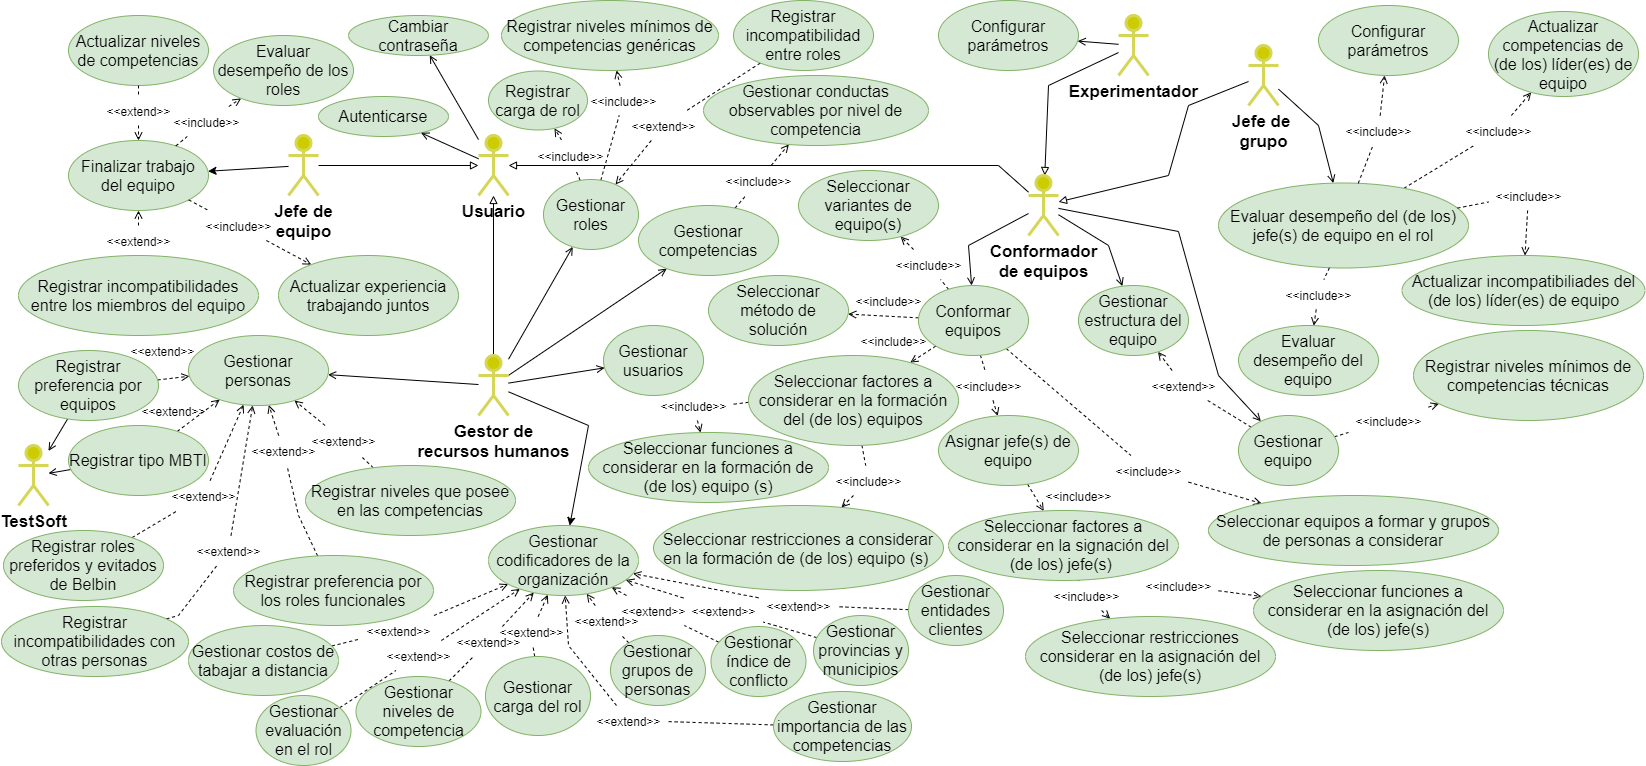
\includegraphics[width=1.2\textwidth]{figuras/diagrama_CUTeamSoft.png} 
	\caption{Diagrama de Caso de Uso del Sistema de TEAMSOFT$^+$. Recreado a partir de \cite{Duran2019}}  \label{fig:cuteamsoft}
\end{figure}

En la Figura \ref{fig:opcines_teamsoft} se observan las opciones implementadas en la herramienta. En la etapa de \textbf{Configuración} se establece las escalas de valores en la que se miden el nivel de cumplimiento de las competencias y los roles. En la opción \textbf{Personal}, se gestionan las competencias, roles y personas. Por último, en \textbf{Proyectos}, se gestionan y se forman los equipos.\\

\begin{figure}[H]
	\centering
	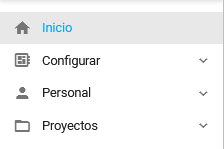
\includegraphics[width=0.4\textwidth]{figuras/opciones_team_soft.png} 
	\caption{Opciones de TEAMSOFT$^+$}\label{fig:opcines_teamsoft}
\end{figure}

El sistema realiza el proceso de asignación del personal en tres etapas. A continuación se explica en qué consiste cada una, y en la Figura \ref{fig:conf_equip_teamsoft} se observa específicamente el paso número dos:
\begin{description}
	\item[Primera etapa:] se configura la cantidad máxima de roles, se elijen los equipos a formar y además los grupos de personas que se van a tener en cuenta para el proceso de formación del equipo.
	\item[Segunda etapa:] se asigna el Jefe de equipo. En esta etapa se toman en cuenta los elementos definidos por el usuario para desempeñar este rol, por ejemplo: competencias técnicas y genéricas, tipos psicológicos, entre otros.
	\item[Tercera etapa:] se forma el equipo. En la asignación del resto del equipo, se tienen en cuenta todas las funciones objetivos y restricciones del modelo.
\end{description}

%El sistema realiza el proceso de asignación del personal en tres etapas (ver figura \ref{fig:conf_equip_teamsoft}), una primera de configuración, donde se establece la cantidad máxima de roles, se elijen los proyectos a formar y además los grupos de personas que se van a tener en cuenta para el proceso de asignación. Las etapas restantes, como propone \cite{Institute2020}, asignan primero al Jefe de Proyecto (segunda etapa) y después, se conforma el equipo (tercera etapa). Al  asignar jefe del proyecto se tienen en cuenta los elementos definidos por el usuario para desempeñar este rol, por ejemplo: competencias técnicas y genéricas, tipos psicológicos, entre otros. En la asignación del resto del equipo, se tienen en cuenta además, las incompatibilidades entre las personas y roles en el proyecto.

\begin{figure}[H]
	\centering
	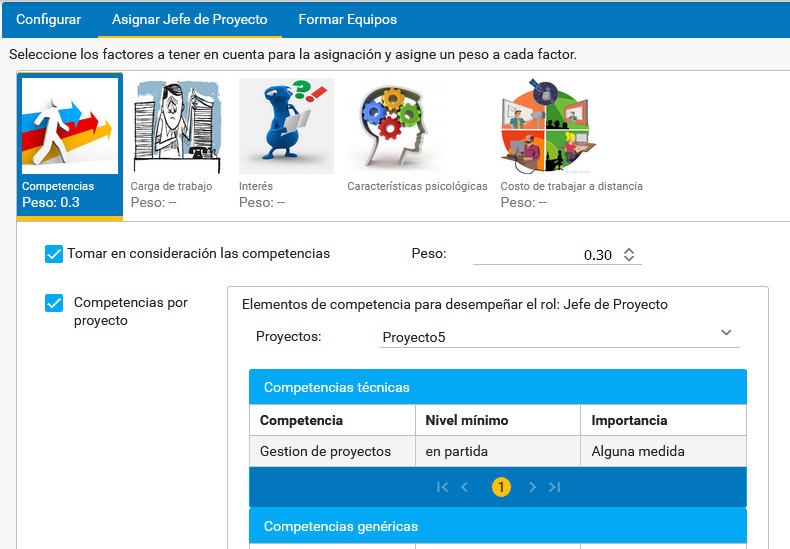
\includegraphics[width=\textwidth]{figuras/conformacion_equipos_asignar_jefe.png}
	\caption{Paso en el que se elige al Jefe del equipo}\label{fig:conf_equip_teamsoft}
\end{figure}

En la Figura \ref{fig:diag-clases} se muestra el diagrama de clases de TEAMSOFT$^+$. La herramienta parte del diagrama de clases existente en BiCIAM para darle solución al problema de múltiples equipos de proyecto. En color amarillo claro se muestran las clases que posee Biciam para dar solución a un problema de optimización. La filosofía de trabajo es la siguiente:
\begin{itemize}
	\item La clase \textit{Problem} es la encargada de manipular el problema.
	\item La clase \textit{Codification} representa la codificación del problema, es quien manipula las restricciones del mismo.
	\item La clase \textit{Constrain} representa cada una de las restricciones del problema.
	\item La clase \textit{State} representa una solución.
	\item La clase \textit{Operator} representa un operador.
	\item La clase \textit{ObjectiveFunction} representa cada una de las funciones objetivo del problema.
\end{itemize}

En color naranja se muestran las clases implementadas en Teamsoft+, las cuales se describen brevemente a continuación:
\begin{itemize}
	\item La clase \textit{TeamFormationProblem} hereda de \textit{Problem} y es la encargada de manipular el problema.
	\item La clase \textit{TeamFormationCodification} representa la codificación del problema y hereda de la clase \textit{Codification} de BiCIAM, y es quien manipula las restricciones del mismo.
	\item La clase \textit{TeamFormationState} representa una solución y hereda de la clase \textit{State} de BiCIAM.
	\item Los operadores de permutación y sustitución heredan de la clase \textit{Operator} de BiCIAM.
	\item Se define una clase para cada una de las funciones objetivo del problema y para cada una de sus variantes balanceadas, que heredan de la clase \textit{ObjectiveFunction} de BiCIAM.
	\item Se implementa una clase por cada una de las restricciones del problema, estas heredan de la clase \textit{Constrain} que representa una restricción.
\end{itemize}

\newpage
\KOMAoptions{paper=landscape, pagesize}
\recalctypearea
%\begin{sidewaysfigure}
	\begin{figure}[H]
%		\centering
\hspace{-3.2cm}
		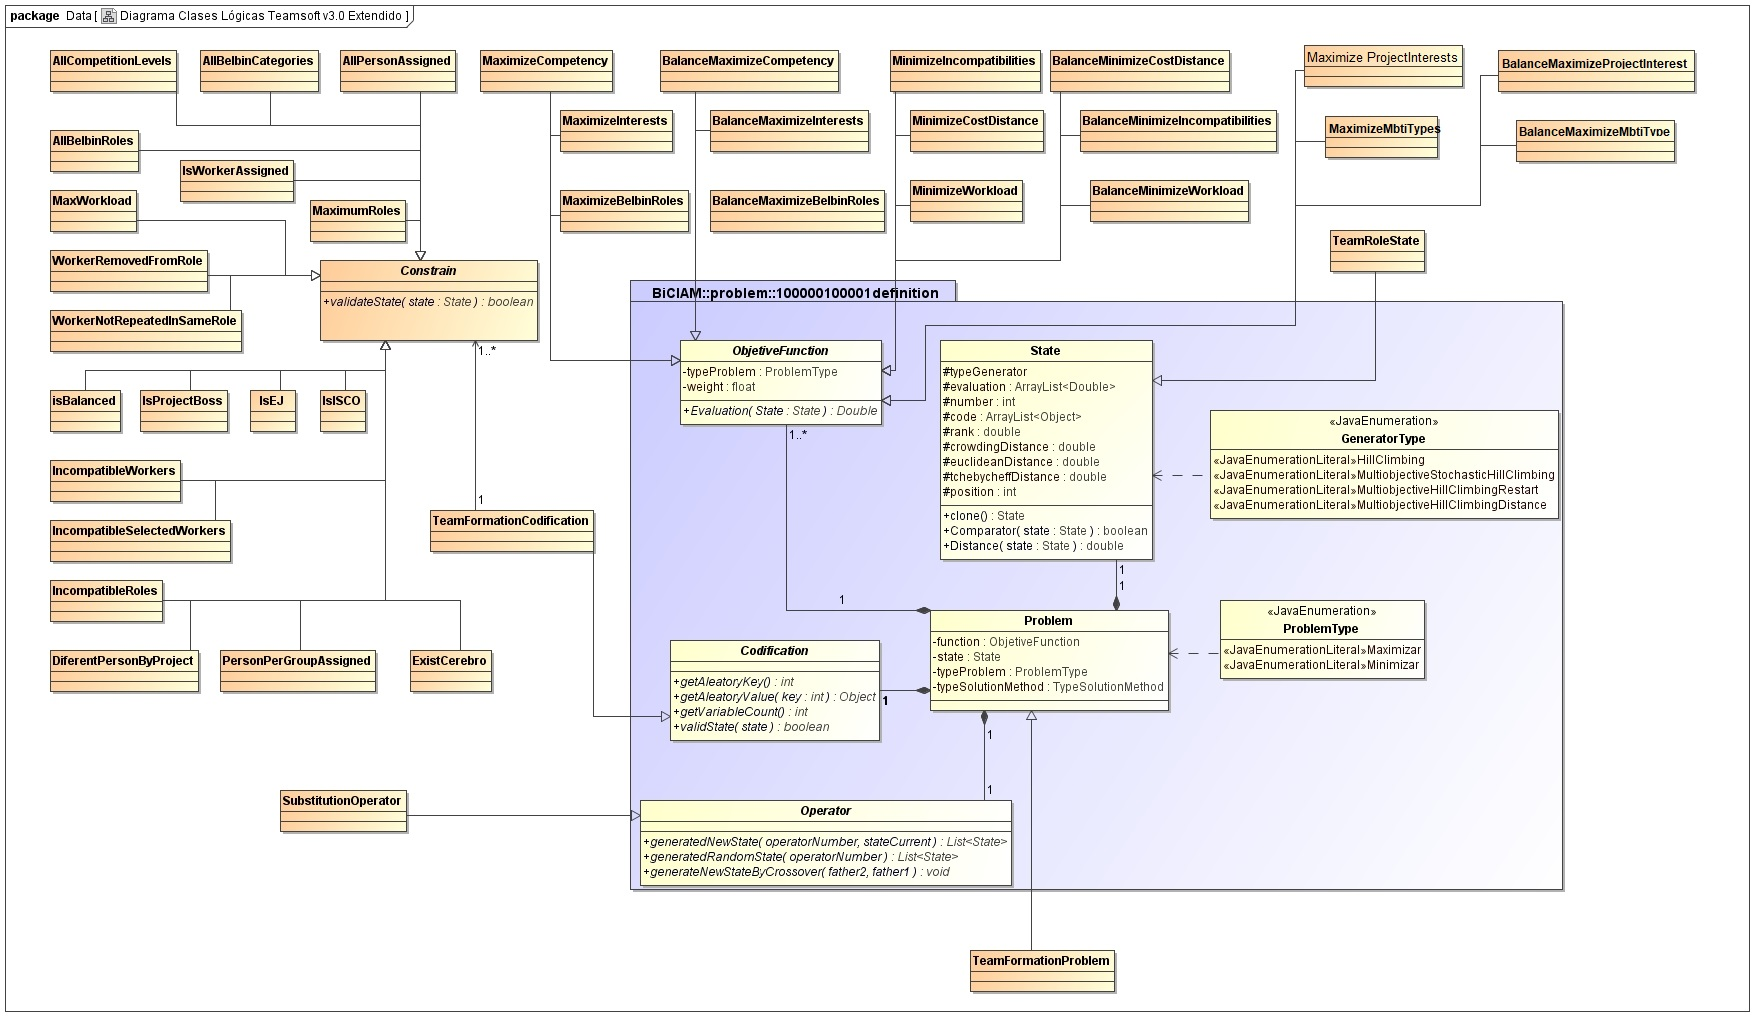
\includegraphics[width=1.3\textwidth]{figuras/diagrama-clases-teamsoft.jpg}
		\caption{Diagrama de clases de TEAMSOFT$^+$}\label{fig:diag-clases}
	\end{figure}
%\end{sidewaysfigure}
\newpage
\KOMAoptions{paper=portrait, pagesize}
\recalctypearea

TEAMSOFT$^+$ utiliza un arquitectura por capas basado en reutilización. En la Figura \ref{fig:diagrama-paquetes} se muestran los paquetes, subsistemas e interfaces que componen dicha arquitectura con distintos niveles de reutilización. 

\begin{figure}[H]
	\centering
	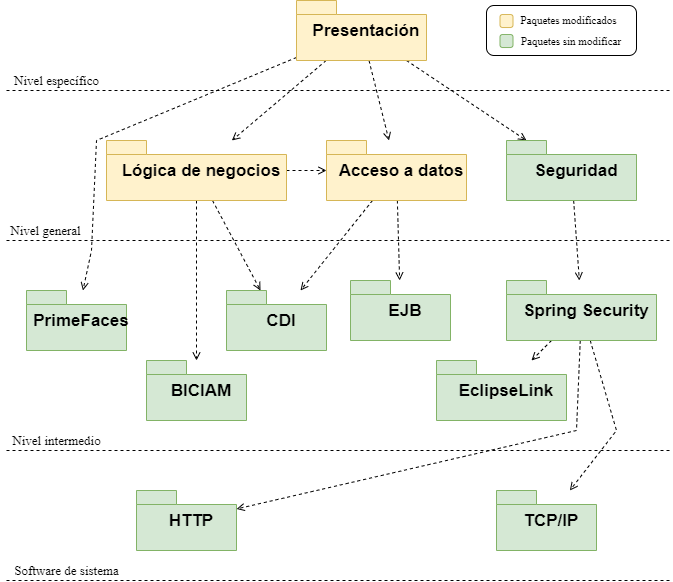
\includegraphics[width=.7\textwidth]{figuras/diagrama-paquetes.png}
	\caption{Diagrama de estructuración en capas basado en reutilización. Recreado a partir de \cite{Duran2019}.} \label{fig:diagrama-paquetes}
\end{figure}

\begin{description}
	\item[Presentación:] Paquete que contiene las páginas XHTML (\textit{Facelets}) y las plantillas (\textit{Templates}) correspondientes a las mismas.
	\item[Lógica de Negocio:] Paquete que contiene las clases que implementan la lógica del negocio. Este paquete agrupa los controladores, objetos java planos (\textit{POJO} por sus siglas en inglés) útiles, y las clases relacionadas con la solución al modelo de formación de múltiples equipos con la biblioteca BiCIAM. 
	\item[Acceso a Datos:] Paquete que contiene las clases para el acceso a datos. Dentro de este se encuentran las \textit{Entity} (clase java con anotaciones, que representa una tabla en la BD), y los modelos (una clase abstracta que define los métodos comunes de creación, actualización y eliminación, y una implementación de esta clase por cada \textit{Entity}) 
	\item[Seguridad:] Paquete que contiene las clases necesarias para la autenticación de los usuarios, validación de identidad y comprobación de permisos. 
	\item[EclipseLink:] Paquete que contiene las clases de la implementación de \textit{JPA}, que permiten el mapeo objeto-relacional. 
	\item[Spring Security:] Paquete que tiene las clases correspondientes al \textit{framework} \textit{Spring Security}, utilizadas en la implementación de la seguridad del sistema. 
	\item[PrimeFaces:] Paquete que contiene las clases necesarias para el uso de los componentes de interfaz de usuario. 
	\item[BiCIAM:] Paquete que contiene las clases necesarias para la utilización de los algoritmos metaheurísticos empleados en la solución al modelo de formación de múltiples equipos. 
	\item[CDI:] Paquete que contiene las clases necesarias para la inyección de dependencias. 
	\item[EJB:] Paquete que contiene las clases necesarias para el uso de componentes empresariales
	\item[HTTP:] Protocolo de Transferencia de Hipertexto, que permite la transmisión de datos. Es utilizado en la aplicación para que los datos viajen de la máquina cliente al servidor web y de este a la máquina cliente. 
	\item[TCP/IP:] Protocolos que conforman la base de Internet, a través de los cuáles se comunica una máquina con otra. 	
\end{description}

El diseño de la base de datos utilizado por la herramienta le da soporte a al modelo de conformación de equipos múltiples. Para más detalles, se puede de consultar el Anexo \ref{fig:diagrama-bd} donde se muestra el diagrama físico de la base de datos.

\section{Formación de equipos de béisbol} \label{ej-pel}

El béisbol es un deporte con una amplia difusión en el continente americano y asiático, e incluso, en los últimos años se ha extendido al continente europeo. Se considera el deporte nacional en países como Cuba y Estados Unidos \cite{INEFI2020}. Dado el auge de este deporte, resulta de gran interés popular la formación de un equipo de béisbol.\\

Un equipo de béisbol está compuesto por varios jugadores. Antes de cada juego, el director del equipo tiene que elegir 10 para la alineación inicial. Cada jugador, con excepción del pícher\footnote{anglicismo aceptado por la RAE para la voz inglés pitcher} y el bateador designado, tiene que desempeñar dos tipos de roles, uno a la defensiva y otro a la ofensiva. En el caso particular del pícher, solo está presente en la alineación defensiva, mientras que el bateador designado ocupa su puesto a la ofensiva. Resulta importante resaltar que un jugador no puede jugar más de un rol del mismo tipo en una alineación. Para cada tipo de rol, existe un conjunto de características o competencias a tener en cuenta para la asignación de un jugador. Por ejemplo, según \cite{Smith1995},  las competencias genéricas a tener en cuenta son:

\begin{itemize}
	\item Trabajo bajo presión (\textit{Peaking Under Pressure}): capacidad del jugador de sentirse desafiado en lugar de amenazado por la presión y su rendimiento bajo presión.
	
	\item Libre de preocupaciones (\textit{Freedom From Worry}): no se presiona a sí mismo, preocupándose por desempeñarse mal o cometer errores. No se ve afectado por las opiniones de los demás con respecto a su desempeño.
	
	\item Afrontar la adversidad (\textit{Coping With Adversity}): permanece positivo y entusiasta, incluso cuando las cosas van mal, permanece tranquilo y controlado; puede recuperarse rápidamente de errores y contratiempos.
	
	\item Concentración (\textit{Concentration}): No se distrae fácilmente; capaz de concentrarse en la tarea en cuestión en tanto en situaciones de práctica como de juego, incluso cuando ocurren situaciones adversas o inesperadas.
	
	\item Preparación mental (\textit{Mental Preparation}): planea y se prepara mentalmente para los juegos y claramente tiene un “plan de juego" para lanzar, batear, correr bases, etc.
	
	\item Motivación para el logro (\textit{Achievement Motivation}): tiene confianza y está motivado positivamente; constantemente da el 100\% durante las prácticas y los juegos; trabaja duro para mejorar sus habilidades.
	
	\item Entrenabilidad (\textit{Coachability}): abierto y aprende de la instrucción; acepta la crítica constructiva sin tomárselo personalmente y enojarse.
\end{itemize}

En el caso de las competencias técnicas a cumplir por un jugador, en una alineación, según \cite{2020a, Silverman2011} son:
\begin{itemize}
	\item Promedio de bateo.
	\item Fuerza de bateo.
	\item Precisión de tiro. 
	\item Fildeo.
	\item Velocidad.
	\item Versatilidad.
\end{itemize}

En la literatura existen diversas investigaciones relacionadas con la formación de equipos de béisbol. En \cite{Polyashuk2015, Sugrue2007} los autores se basan en las estadísticas de los jugadores almacenadas a lo largo de los años para construir un indicador. En base a este indicador es que se realiza el proceso de asignación de los jugadores a los roles. Las investigaciones planteadas anteriormente, solo se enfocan en la formación de la alineación ofensiva (orden al bate), sin tener en cuenta la alineación defensiva. Además, no tienen en cuenta las competencias que necesitan los roles para ser ocupados, y tampoco hacen referencia a la preferencia de las personas por los roles.

\section{Formación de equipos docentes} \label{ej-carga}

La planificación de la carga docente es un problema recurrente en cada inicio de semestre para los encargados en cada centro de educación. En el proceso de asignación de la carga docente intervienen dos aspectos fundamentales: el claustro de profesores disponibles y el conjunto de asignaturas a impartir.\\

En \cite{res2018} se define cómo organizar el proceso docente de cada asignatura, siendo imprescindible conocer, la cantidad de horas asociadas a cada forma de enseñanza, estas son:
\begin{itemize}
	\item Conferencia(C)
	\item Clase práctica(CP)
	\item Seminario(S)
	\item Laboratorio(L)
	\item Taller(T)
\end{itemize}

Cada forma de enseñanza se puede considerar como los roles a desempeñar por los profesores en el colectivo de asignatura. Cada uno de estos roles tiene asociado un conjunto de competencias que debe satisfacer el profesor para desempeñarlo correctamente. Por ejemplo \cite{res2016} recomienda que las conferencias sean impartidas por un profesor de experiencia, entre otros aspectos.\\

Del claustro de profesores se conocen sus competencias, preferencias y disponibilidad. Por ejemplo: la categoría docente y científica, los años de experiencia impartiendo las asignaturas, el fondo de tiempo disponible para la docencia y, el interés por las asignaturas, entre otras. Las categorías docentes que puede alcanzar un profesor están definidas en \cite{res2016}, estas son:
\begin{itemize}
	\item Profesor Titular
	\item Profesor Auxiliar
	\item Profesor Asistente
	\item Instructor
\end{itemize} 

El jefe de departamento es el encargado de elaborar el Plan de resultado de cada profesor y, al finalizar el año verificar su cumplimento. En función del cumplimiento del plan, se le otorga a cada profesor una evaluación general. La evaluación general se otorga a partir de un consenso entre las siguientes seis dimensiones \citep{Ansola2020}:
\begin{itemize}
	\item \textbf{Docente}. Clases impartidas (cantidad de grupos y asignaturas, tipos de clase) así como la calidad de ellas. Las tutorías de tesis y prácticas profesionales.
	\item \textbf{Metodológico}. Cumplimiento del Plan Metodológico de la Asignatura (planificación de las clases y otras actividades), cumplimiento del Plan de Controles a Clases del Departamento.
	\item \textbf{Superación}. Cambio o ratificación de categoría docente, cursos de superación o postgrado.
	\item \textbf{Investigación}. Publicaciones en revistas, libros, premios.
	\item \textbf{Extensión universitaria}. Participación en: donaciones de sangre, juegos 13/3 para trabajadores, cuidado de Pruebas de Ingreso a la Educación Superior, entre otras actividades que se puedan realizar en la Universidad.
	\item \textbf{Política}. Actitud ante los estudiantes y resto de los compañeros, cumplimiento de la Guardia Obrera, participación en actividades políticas y de masa organizadas por la Universidad o el país. Pertenencia a organizaciones políticas (UJC-PCC).
\end{itemize}

Muchas universidades del mundo tienen que enfrentar el proceso de asignar profesores a los tipos de clases que le corresponden a las asignaturas, al menos una vez al año. En la literatura existen múltiples investigaciones que se enfocan en la asignación de los profesores a las asignaturas. Por ejemplo, en \cite{Domenech2014} se presenta un modelo donde se realiza el proceso de formación del equipo asignando los profesores a las asignaturas. Este trabajo tiene en cuenta el balance de la carga de los profesores y sus preferencias hacia las asignaturas. En \cite{Bosquez2020} se propone otro modelo para la asignación de asignaturas a profesores, basándose en la preferencia de los mismos hacia las asignaturas (si le interesaba darla o no). En ninguno de los trabajos revisados los autores tienen en cuenta para realizar la asignación, las competencias de los profesores, ni las competencias necesarias para cada cumplir cada rol. Tampoco hacen referencia a las incompatibilidades que pueden existir entre los miembros del colectivo de una asignatura.

\section{Conclusiones parciales}
Una vez terminado el capítulo se arriban a las siguientes conclusiones:
\begin{enumerate}
	\setlength\itemsep{0em}
	\item Existe un modelo definido para el problema de formación de equipos de software que tiene propiedades generales, debido a que incluye personas, roles, competencias.
	\item Existe una herramienta que le da soporte al modelo de formación de equipos de software denominada TEAMSOFT$^+$.
	\item Para los problemas de formación de equipos docentes y de béisbol no existen modelos definidos que tengan en cuenta las competencias de las personas para ocupar los roles, las incompatibilidades entre las personas y las preferencias por los roles.
	\item Tanto el modelo como la herramienta TEAMSOFT$^+$ podrían se aplicados para formar equipos docentes y de béisbol, ya que toman en cuenta los factores a considerar en cada caso.
\end{enumerate}
\pagebreak
%\subsection{Requisitos funcionales}
%\begin{itemize}
%	 \item Realizar la modelación de los datos correspondientes a lo descrito en la sección \ref{chap:descripcion}, incluyendo un nombre para cada entidad descrita.
%	\item Desarrollar la base de datos que se corresponde con el modelo identificado.
%	\item Implementar la carga de datos a partir de un fichero de entrada, para otorgar valores a los conjuntos descritos en la sección \ref{entidades}.
%	\item Importar y exportar la base de datos.
%\end{itemize}
%\subsection{Requisitos no funcionales}
%\begin{itemize}
%	\item La interfaz deben mantener un mismo patrón de diseño que resulte comprensible al usuario. 
%	\item Utilizar un método para el control de versiones.
%\end{itemize}
%
%%\section{Conclusiones parciales}
%%Al terminar de leer el capítulo se puede concluir que:
%%\begin{itemize}
%%	\item Con el trabajo rela.
%%\end{itemize}